\section{The shadow}
\paragraph{Ledger.} For a fixed rule and pair, the 64 impact offsets form a uniform input set
($H(I)=6$ bits), and the dynamics is deterministic, so all entropies below are exact for that
ensemble. Let $O$ be the description (species, internal state, position) of all outgoing coherences at
$t=600$. Since the full state determines the input, $H(I\mid O)$ is exactly the information the
background holds and the coherences do not: the \emph{shadow-only} information.

\paragraph{Intervention.} At $t=600$ every resolved coherence is erased (both layers set to vacuum),
leaving only the residue. A probe, an exact copy of the right-moving object's free-flight state, is
written at one fixed site outside every shadow for all 64 offsets, so its starting position carries no
information about the input. The worlds with and without the probe are run for 1500 further ticks.
The \emph{footprint} $Y$ is their difference. The \emph{probe state} $Y_p$ is the set of resolved
coherences in the region where they differ. We report $I(I;Y\mid O)/H(I\mid O)$ and
$I(I;Y_p\mid O)/H(I\mid O)$.

\paragraph{Results.} The null holds exactly: in all \nsthreeClean{} pairs whose background
returns to vacuum after erasure, both readouts are zero. In all \nsthreeShadow{} pairs that leave a
residue (\nsthreeShadowRules{} rules) the footprint ratio is exactly 1. The probe's passage
determines every bit of the shadow-only information, which ranges from \nonlyMin{} to
\nonlyMax{} bits (Fig.~\ref{fig:ledger}, left). The record is also often carried out by a coherence:
the probe-state ratio is positive in \nsthreeStatePos{} of \nsthreeShadow{} pairs and equal to 1 in
\nsthreeStateOne{}, with median \nsthreeStateMed{} (Fig.~\ref{fig:ledger}, right). A coherence of the
probe's own species leaves in a median of \nsurvMed{} of 64 runs. All shadow rules have an active
vacuum. An earlier one-pair-per-rule version of the test (\nstwoShadow{} shadow rules, \nstwoClean{}
clean) gave the same footprint result.

\begin{figure}[t]\centering
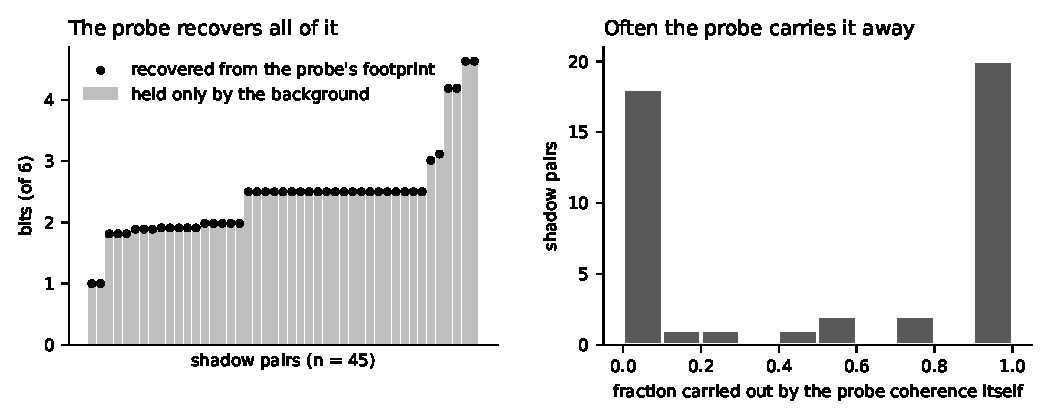
\includegraphics[width=\linewidth]{figures/fig3_ledger.pdf}
\caption{Left: information held only by the background after a collision (bars) and the amount
recovered from a probe's footprint after the carriers were erased (dots), for every shadow pair.
Right: fraction of that information carried out by the probe coherence itself.}\label{fig:ledger}
\end{figure}
